\subsection{Mathematical Preliminaries of Statistical Mechanics}
\label{sxn:mathP}

%MM% We will compare and contrast the several types of energies and averages we will encounter:
%MM% Thermal Averages (over the weights $\WVEC$),
%MM% Sample Averages (over the data $\XVEC$),
%MM% and \FreeEnergies and \GeneratingFunctions.
%MM% We will define the different averages, 
%MM% show how they are related to each other under the  \AnnealedApproximation (AA) and in the \HighTemperature (High-T) limit,
%MM% and explain how and when may use the (overloaded) \BraKet notation $\langle \cdots \rangle$ for the different averages.
%MM% We will then show how to compute the average training and test/generalization errors $\AVGTE, \AVGGE$
%MM% using the \FreeEnergy as a \GeneratingFunction, and how they are related to each other
%MM% in the AA and the High-T limit.  We  briefly define \Replicaa Averages and
%MM% also the \SaddlePointApproximation (SPA).
%MM% Finally, we review how to express the \FreeEnergy
%MM% as a matrix-generalized \ThermalAverage over random matrices, called an HCIZ integral.

\paragraph{SubSection Roadmap}
Briefly, in the following subsection,
we start by defining an arbitrary NN model, with weights $(\WVEC)$.
Then, we explain the difference between using real-world $(\XVEC)$ and random data $(\XI)$.
This lets us define an energy error function, $\DETOP$,
the error the NN makes on the data.
We then explain how to take different kinds of \emph{\Thermodynamic} averages of the data,
including \emph{Sample} and \emph{\ThermalAverages} and the implications,
and the difference between computing errors and accuracies.
Next, we define the \emph{FreeEnergy} $(F)$ for the error(s), and the \emph{GeneratingFunction}  $(\Gamma)$
for the accuracy and/or quality.
From here, we explain the \emph{AnnealedApproximation} (AA) and
how to define the  \emph{\AnnealedHamiltonian}, $\GAN$, a crucial expression
that will be the starting point later for our matrix model.
In the AA, $\GAN$ simplies to  $\HANHT=\EPSLw$, where $\EPSLw$ is an \EffectivePotential
that depends only on the weights $\WVEC$.
Likewise, we can define the \SelfOverlap, $\ETAw:=1-\EPSLw$, which is useful for
obtaining the \Quality.
We show how to obtain the \emph{Average Training and Generalization Errors} $\AVGTE$, $\AVGGE$
using the \STATMECH formalism, which defines them in terms of partial derivatives of the \FreeEnergy $(F)$.
Doing this, we show that in the AA and at high-T they are equivalent,
$[\AVGSTTE]^{an,hT}=[\AVGSTGE]^{an,hT}$,
and can both be expressed as a \ThermalAverage over all Students, as a function 
of the \Teacher, as $[\AVGSTGE]^{an,hT}=\THRMAVG{\GANHTR}=\THRMAVG{\EPSL(R)}$.
Note that these averages are obtained by using the \FreeEnergy as a \GeneratingFunction.
We then explain how to obtain the \ModelQuality  as  partial derivatives of a
\emph{\GeneratingFunction} $(\Gamma_{\Q})$.
We then discuss the more advanced techniques, the
\emph{\LargeN Approxmation} and the \emph{SaddlePointApproximation} (SPA),
which will be used extensively later.
Finally, we introduce  HCIZ integrals, which will be necessary to evaluate the matrix-generalized
form of $\Gamma_{\Q}$ to obtain the final result.
%\footnote{This assumes that agreement of \Student and \Teacher predictions will follow from overlap of weight vectors --- as it 
%surely does in the \emph{\LinearPerceptron} case, and does with high probability under Lipschitz 
%smoothness~\cite{neyshabur18_TR}. 
%\michaeladdressed{@charles: Im not sure what this is saying.}\charles{YOU WROTE THIS!}
%}
\michael{@charles: What precisely is Accuracy versus Quality?}
\charles{@michael: We have discusses this multiple times. }
%We also degfine  write an expression for the Average \GeneralizationAccuracy,
%$1-\AVGSTGE$, which we call the \ModelQuality.
\michaeladdressed{This last sentence is an exaple of one where the phrasing is a little unclear.  I think we can mention \ModelQuality, but it's not clear if this is from SST or something we introduce, etc.  So, it's unclear later when we use it without a clear definition, etc., in the vector or matrix case.  Probably it's best just to either remove a sentence like that here (if SST did not have it, since here we are describing the past), or have a footnote saying that we will use the \GeneralizationAccuracy they used, but in a different way by considering one-minus it, and then have an explicit pointer to where we define it.}

In this subsection, we will compare and contrast several types of averages and energies we will encounter. 


\begin{enumerate}[label=4.2.\arabic*]
\item
  \textbf{Setup.}
  In Section~\ref{sxn:mathP_setup}, 
we will start by describing the basic setup of the problem, including the distinction between the actual training process and how we model the training process.

 \item
 \textbf{BraKets, Expected Values, and Thermal Averages.}
In Section~\ref{sxn:mathP_averages}, 
we will describe our use of physics BraKet notation for both Sample Averages (over the data $\XVEC$) and Thermal Averages (over the weights $\WVEC$) and ---in particular, under the \AnnealedApproximation (AA) and in the \HighTemperature (High-T) limit---showing how they relate to each other and to the notion of \Replica Averages.
%
\item
  \textbf{Free Energies and \GeneratingFunctions.} 
In Section~\ref{sxn:mathP_free_energies}, 
we will make a connection between these different averaging notions and \FreeEnergies and \GeneratingFunctions, showing how they relate to each other.
%

\item
  \textbf{The Annealed Approximation (AA) and the High-Temperature Approximation (high-T).}
  In Section~\ref{sxn:mathP_annealed}, we explain the \AnnealedApproximation, the \HighTemperature approximation,
  and the Thermodynamic \LargeN limit and the Saddle Point Approximation (SPA).
  We also introduce the \Quality \GeneratingFunction $\Gamma_{\Q}$%
  \item
    \textbf{Average Training and Generalization Errors and their \GeneratingFunctions.}
  In Section~\ref{sxn:mathP_errors}, we will show how to compute the Average Training and Test/Generalization Errors $\AVGTE, \AVGGE$
using the \FreeEnergy as a \GeneratingFunction, and how these errors are related to each other in the AA and High-T limit. 
%
\item 
  \textbf{The Thermodynamic limit.}
  In Section~\ref{sxn:largeN_and_SPA}, we discuss the \LargeN \ThermodynamicLimit and the \SaddlePointApproximation (SPA),
  along with the concepts of \SelfAveraging and \WickRotations.
%
\item 
  \textbf{From the ST Perceptron to a Matrix Model.} 
  Finally, in Section~\ref{sxn:from_vectors}, we introduce the physical concepts necessary to understand the \SETOL matrix model, including the \WideLayer \LargeN limit and the notion of \SizeConsistency.  We  then describe how to obtain the \LayerQuality $\Q$ from a matrix-generalized \ThermalAverage over random matrices, called an HCIZ integral.
\end{enumerate}
The various symbols and other important results are summarized in the Appendix~\ref{sxn:appendix_A}


\subsubsection{Setup}
\label{sxn:mathP_setup}

A basic issue in formulating \SETOL is that one typically trains one large (expensive) NN, i.e., one does not necessarily  need to split the data into training and testing sets (as in more traditional hyperparameter tuning of ML models).
Thus, we want a methodology to approximate quantities such as the generalization error or generalization accuracy that does not rely on traditional train-test splitting methods.
\michaelB{Q: how does this lack of using training/testing split relate to that we ignore the $y$ below and/or that we are actually getting a notion of quality/accuracy, rather than error (related to $\Gamma_{\red{\ND}}$ versus $F_{\red{\ND}}$).}
To accomplish this, we idealize the empirical data distribution as Gaussian fields, and we will use \STATMECH to construct quantities (basically, free energies or generating functions) so that we can compute training/testing errors by taking appropriate derivatives of these quantities.

In more detail, we imagine training a NN on $\ND$ training data instances, $\XVEC_{\mu}$, which are $m$-dimensional vectors,
with labels $y_{\mu}$, chosen from a large but finite-size training data set $\ADD$.
The goal of training a perceptron (or, later, a NN) is to learn the $m$ weights of the vector $\WVEC$ (or, later, a weight matrix $\WMAT$) by running a form of stochastic gradient descent (SGD) to minimizing a loss function $\mathcal{L}$ ($\ell_2$, cross-entropy, etc.). 
We want to approximate the actual network’s learning dynamics by an analytically tractable ensemble
so that we can then obtain 
analytic expressions for the \emph{\FreeEnergy} and \emph{\GeneratingFunction} we then use to compute
Thermodynamic averages such as the \emph{\AverageGeneralizationError} $(\AVGGE)$ and
\emph{\ModelQuality} $(\Q)$ (which is our approximation to the \emph{\AverageGeneralizationAccuracy}).


\begin{figure}[t] %[h] % [h] places the figure approximately here
    \centering
\resizebox{0.75\textwidth}{!}{
\begin{tikzpicture}[
     thick, % Line thickness
    rectnode/.style={rectangle, draw=black, thick, minimum width=6cm, minimum height=2.5cm, rounded corners=0.3cm}, % Rectangular node style with rounded corners
    -> % Arrow style
]

% Nodes with manual positioning
\node[rectnode] (realdata) at (0,0) {%
    \begin{minipage}{6cm}
        \centering
        \textbf{Real Data} \\
        \vspace{0.3cm}
        $\mathbf{x_\mu}, \mathrm{y}_\mu \in \mathbf{D},\;\mu=1, 2, \ldots, n$\\
        $\text{where }$ \\
        $\mathrm{y}_\mu \in \{-1, 1\}$ \\
        $\mathbf{x_\mu}\text{ is real world, correlated data }$ \\
        $\mathbf{x_\mu} \in \mathbb{R}^{M}$, $\Vert\mathbf{x_\mu}\Vert^{2}_{F}=1$
    \end{minipage}
};

\node[rectnode] (modeldata) at (8,0) {%
    \begin{minipage}{6cm}
        \centering
        \textbf{Idealized Data} \\
        \vspace{0.3cm}
        $\boldsymbol{\xi}_\mu, y_\mu \in \mathbf{\mathcal{D}},\;\mu=1, 2, \ldots, \infty$ \\
        $\text{where }$ \\
        $y_\mu \in \{-1, 1\}$ \\
        $\boldsymbol{\xi}_{\mu} \sim \mathcal{N}(0, \tfrac{1}{M} \mathbb{I})$ \\
        $\boldsymbol{\xi}_{\mu}\in \mathbb{R}^{M}$, $\Vert\boldsymbol{\xi}_{\mu}\Vert^{2}_{F}=1$
    \end{minipage}
};

% Arrow between the boxes
\draw[->] (realdata) -- (modeldata);

\end{tikzpicture}
}
\caption{Mapping from a fixed set of $n$
  real-world, correlated data instances $[\mathbf{x},\mathrm{y}]\in\mathbf{D}$
  to an uncorrelated, random model of idealized data   $[\boldsymbol{\xi}, y]\in\mathbf{\mathcal{D}}$, drawn from a Gaussian i.i.d. distribution.
}
    \label{fig:data_mapping}
\end{figure}


\paragraph{Counting Samples and Features.}
We let the number of training samples be $\ND$ and the dimension 
(i.e., number of features) for each sample be $m$.
% For simplicity, we also use $\ND$ (instead of $\ND$) and $M$ (instead of $m$), recognizing that 
% \emph{in later sections} $\ND$ and $M$ will refer to the dimensions 
% of a layer’s weight matrix (i.e., an $N \times M$ matrix). 
% We stress that here, in this subsection,  $n = N$ and $m = M$ only hold for our immediate analysis, 
% to avoid extra notation. 
When we move to matrix-based analyses, 
%we will revisit (and possibly distinguish) $\ND$ (layer input dimension) and $\ND$ (training-set size).
the input dimension $m$ will become $M$ and we will induce a new output dimension $\ND$, (the output dimension of a perceptron is $1$). Thus, the layer weight matrix $\WMAT$ has dimension $M\times N$.\footnote{To be more precise, $M$ is defined to be the lesser dimension of $\WMAT$ and $N$ the greater. For simplicity we assume that $M$ is always the input dimension and $N$ the output dimension. Under the assumptions of \SETOL, there is no loss of generality from doing this.} The number of data samples will remain $\ND$ throughout.
\begin{table}[H]
\centering
\begin{tabular}{l|l|l}
\toprule
 \textbf{Definition} & \textbf{Vector} & \textbf{Matrix} \\
\midrule
 Total number of data samples used in training. & $\ND$ & $\ND$ \\
 Number of features per training sample (Input dimension). & $m$ & $M$ \\
 Dimension of layer output (Output dimension)  & $1$ & $N$ \\
 Number of free parameters & $1$ & $N\times M$ \\
 Total number of degrees of freedom & $\ND\times 1$ & $\ND\times N\times M$ \\
\bottomrule
\end{tabular}
\caption{In the \emph{vector} model, lowercase $m$ is the dimension of the weight vector (total parameters), which is also the number of features per sample. In the vector case, there is one free parameter -- the overlap $R$ (or angle $\theta$) between student and teacher. In the \emph{matrix} model, uppercase $N$ and $M$ are the input and output dimensions of the weight matrix, resp., giving $N\times M$ free parameters.
The total number of degrees of freedom is the number of training examples $\ND$ times the number of free parameters.}
\label{tab:dim_notation}
\end{table}




\paragraph{Actual and Idealized Data and Energies.}

Consider having a large set $\ND$ of actual, real-world data, 
\begin{align}
  \label{eqn:x}
  \left( \XVEC_{\mu}, \MY_{\mu} \right) \in\ADD,\;\mu=1, \cdots, \ND,
\end{align}
where 
$\XVEC_{\mu}\in\mathbb{R}^{m}$ is an $m$-dimensional real vector, 
$\MY_{\mu}$ is a binary label taking values $\{-1,1\}$, and 
$\ADD$ denotes the finite-size dataset.
WLOG, we assume that $\XVEC_{\mu}$ is normalized such that the norm squared is unity:
\begin{equation}
  \label{eqn:XVEC_norm}
  \Vert\XVEC_{\mu}\Vert^{2} := \sum_{i=1}^{m} \XVEC_{\mu,i}^{2}=1
\end{equation}
We call $\XVEC^{\ND}$ an $\ND$-sized sample (of the training data instances $\XVEC$) from $\ADD$. 
% See below We may or may not specify the labels for this sample, depending on the context.

We define model errors
as an energy $\Delta E^{\red{2}}_{\mathcal{L}}$, the difference squared between the student's and teacher's output, since their outputs are a form of energy.
Smaller energies correspond to smaller errors and therefore better models.
For example, for the mean-squared-error (MSE) loss, one has
\begin{align}
  \label{eqn:DEy}
  \DEL(\WVEC,\XVEC_{\mu},\MY_{\mu}):= (\MY_{\mu}-\NNOUT(\WVEC,\XVEC_{\mu}))^{2}  ,
\end{align}
where $\NNOUT(\WVEC,\XVEC_{\mu})$ is output prediction of the NN, as in \EQN~\ref{eqn:dnn_energy}.
\footnote{The function $\NNOUT$ is not an energy  in the sense for this work.}


We assume that there is a real-world training process that generates a \Teacher model $(T)$, trained on a particular dataset $\ADD$, and we seek a theory for the \Quality (or generalization accuracy) of this model.
 To estimate quantities such as the generalization error or generalization accuracy, we will adopt an approach that starts off by assuming idealized Gaussian data $\MDD$, 
 but ends with  the NN with a parametric model that we will fit with a \SemiEmpirical procedure (described later).
 To that end, in the theoretical setup,
%In particular, a core assumption of the \SETOL is that $\MY_{\mu}$ is also the output of a (realizable) Teacher NN. Thus, as we will see below, $E_{\mathcal{L}}$ is defined with reference to the Teacher weights, rather than the labels $\MY_{\mu}$, leading $\MY_{\mu}$ to be dropped from expressions of the error. This, and the fact that we will integrate out the data terms, are among the reasons why \SETOL is able to offer data-independent model Quality metrics. 
the replacement scheme is,
\begin{align}
\label{eqn:model_real_world_expt}
  \ADD \rightarrow \MDD,\;\;\XVEC_{\mu} \rightarrow \XImu,\;\;  \Ymu \rightarrow y_{\mu}  ,
\end{align}
where we denote the model training and/or test data instances as $(\XI,y)$ 
such that
\begin{align}
    \label{eqn:xi}
  \left(\XI_{\mu}, y_{\mu} \right) \sim \MDD,\;\mu=1, \cdots, \infty  .
\end{align}
Here, $\XImu\in\mathbb{R}^{m}$ is a random vector (i.e., an $m$-dimensional random variable), sampled from an i.i.d $m$-dimensional joint distribution $\MDD$ of both the features $\XI_{\mu}$, which are Gaussian, and the labels $y_{\mu}$, which are binary NN outputs. Since we assume that the labels are fixed, and the labels are deterministically generated by it, $\MDD$ is effectively just the \emph{idealized} Gaussian feature distribution.
%

\subsubsection{BraKets, Expected Values, and Thermal Averages}
\label{sxn:mathP_averages}
Given the setup from Section~\ref{sxn:mathP_setup},
we will treat the total energy, $\DETOPX$, over some $\ND$-size data set $\NDX$.
we can write the \TotalDataSampleError,
using an overloaded operator notation, as
\begin{align}
  \label{eqn:detopxy}
  \DETOPXY :=\sum_{\mu=1}^{\ND}\DEL(\WVEC,\XVEC_{\mu}, \MY_{\mu})  ,
\end{align}
where the boldface $\DETOP$ indicates this is a sum over the entire set of $\ND$ pairs $[\NDX, \MY^{\ND}]$.
 We should keep in mind that this depends on the specific set of $\ND$ data pairs $[(\XVEC_{\mu},\MY_{\mu})\in\ADD\;|\;\mu=1,\cdots,n]$, 
 although later we will model the labels $\MY_{\mu}$ as the output of another NN when describing the Student-Teacher model.
Doing so later, here, we treat $\MY_{\mu}$ as a deterministic output of the Teacher model $T$, meaning that
$\MY_{\mu}$ is \emph{implicit} in $\DEL$.
We will therefore drop the $\MY_{\mu}$ and $y^{\ND}$ symbols, 
and simply write this total error / energy difference as
\begin{align}
  \label{eqn:detox_FIXLATER}
  \DETOPX :=\sum_{\mu=1}^{\ND}\DEL(\WVEC,\XVEC_{\mu})  ,
\end{align}
which is now a function of the entire set of $\ND$ vectors $[\NDX]$.%
% (where the labels $\MY$ have been set implicitly).
\footnote{In the classic Student Teacher model, the labels  $\MY^{\ND}$ represent the Teacher outputs and are effectively treated as either uniform random variables to be averaged over later, or as the outputs of an optimal Teacher. In this work, the Teacher is fixed so we can drop the labels.}
This operator notation will prove useful later in Section~\ref{sxn:SMOG_main-st_av}
(see \EQN~\ref{eqn:DE_L}) and in Appendix~\ref{sxn:summary_sst92}.

We will not, however, work directly with samples and sample averages.
Instead, we will model them.
%%\michael{By that, I think we mean that it is hard to compute them, so we will model them with Gaussian random variables with a model with a parameter to fit semi-empirically to data; correct?}
%%\cformike{We discussed on the phone.  The idea is we compute the average as a derivative of a generating function that we know exactly, as opposed to say doing a monte carlo sample because the partition function $Z_{\red{\ND}}$ is intractable}
To that end, we need to estimate them with a theoretical approach. For example, we can write the \TotalDataSampleError 
in terms of our random data variables $\NDXI$, written formally as
\begin{align}
\label{eqn:tdse}
\DETOPXI := \sum_{\mu=1}^{\ND}\DETmu ,
\end{align}
but to evaluate this we need to take an integral and/or \ExpectedValue over the data sample $\NDXIn$.

\paragraph{Expected Values.}

We need to compute various sums and integrals, sampling from a \emph{idealized} $\MDD$ for the \emph{actual} (i.e, real-world) data distribution $\ADD$,  over $\ND$-sized data samples (or data sets), and also over distributions of weights ($\WVEC, \SVEC$) and weight matrices ($\WMAT, \SMAT, \AMAT, \cdots$).
This will frequently (but not always) be defined as more familiar \ExpectedValues.
We will denote \ExpectedValues using physics \BraKet notion.
Importantly, we use the term \ExpectedValue in the physics sense, and BraKets will denote an un-normalized sum or integral;
%notation denotes an inner product in a Hilbert space of functions;
when the quantity is to be normalized, we will denote the normalization explicitly.
For example, given a function $f(\XI)$, we write the BraKet integral as:
\begin{align}
 \label{eqn:EuT}
 \langle f(\XI) \rangle_{\XI}:=\int d\mu(\XI) f(\XI)  .
\end{align}
We would express an $\ND$-sized sample average over $f()$ as 
\begin{align}
    \label{eqn:EuT_normalized}
    \langle f(\NDXIn) \rangle_{\AVGNDXIn} :=& \frac{1}{\ND} \int d\mu(\NDXIn) f(\NDXIn) \nonumber \\
    =& \frac{1}{\ND} \left[\prod_{\mu=1}^{\ND} \int d\XI_{\mu}P(\XI_{\mu}) \right] \left[ \sum_{\mu=1}^{\ND}f(\XI_{\mu}) \right].
\end{align}
The BraKet $\langle\cdots\rangle_{\AVGNDXIn}$ denotes an integral over an $\ND$-sized sample of idealized
Gaussian-field data $\NDXIn$, with the convention that summation over $\ND$ points and normalization $\tfrac{1}{\ND}$
appears inside the \BraKet implicitly.

For example, we treat an \ExpectedValue of the \DataSampleError , which is correlated when using real-world data $\ADD$, using the uncorrelated idealized data $\MDD$; this is specified with the following mapping:
\begin{align}
  \label{eqn:Emap}
  \frac{1}{\ND}\DETOPX \xrightarrow{\text{Expected Value}} \langle \DETOPXI \rangle_{\AVGNDXIn}  , %= \DETOT = n \EPSLw.
\end{align}
where the BraKet $\langle\cdots\rangle_{\AVGNDXIn}$ deotes the integral over the idealized dataset $\NDXIn$, but with the convention that the normalization $\tfrac{1}{n}$
appears inside the \BraKet implicitly.
In this case, we obtain:
\begin{align}
\nonumber
  \langle \DETOPXI\rangle_{\AVGNDXIn}
  :=  &\frac{1}{\ND}\int d\mu(\NDXIn) \DETOPXI \\ 
  = &
  \frac{1}{\ND}\int \left[ \prod_{\mu=1}^{\ND}d\XI_{\mu}P(\XI_{\mu})\right] \left[ \sum_{\mu=1}^{\ND}\DETmu \right] , \\ \nonumber
  = &
  \frac{1}{\ND}\sum_{\mu=1}^{\ND}\int d\XI_{\mu}P(\XI_{\mu})\DETmu  , 
    \label{eqn:average_data_sample_error}
\end{align}
where $P(\NDXIn)$ is a product of $\ND$ i.i.d. $m$-dimensional Gaussian distributions.
The subscript $\AVGNDXIn$ indicates this is an
\ExpectedValue of an average of an $\ND$-size \emph{sample} of ideal data, where the \ExpectedValue is taken over datasets, and the average is over data points within each sample. The third line follows because the $\ND$ samples are i.i.d.
(This is used in both Sections~\ref{sxn:SMOG_main} and~\ref{sxn:matgen}.)
The normalization $\tfrac{1}{\ND}$ ensures the \BraKet is a proper \ExpectedValue of a sample average.
The measure $d\mu(\NDXIn)$ 
denotes the probability measure associated with a single 
\emph{realization} of a random data sample of size $\ND$ drawn from an $m$-dimensional idealized Gaussian distribution.
A subscript $\XI$ on the Ket as $\langle\cdots\rangle_{\XI}$ indicates that the integral over potential data points, not an average of a data sample (i.e., there would be no $1/\ND$ prefactor).
% \michaeladdressed{@charles: clarify; that is $\ND$ vectors in $\mathbb{R}^{M}$ that are element-wise i.i.d. Gaussian?}
%%\michael{Where we are using $M$ and $\ND$ rather than $m$ and $\ND$; is that a typo, or what should it be.}
%%\cformike{I use $n,m$ in this section, $\ND$, $M$ elsewhere since they can mean different things when we generalize to a layer.  We can fix if its too confusion, or maybe just explain above.}
%

\paragraph{\SizeExtensivity and \SizeIntensivity}
A key requirement for the \ThermodynamicLimit in \STATMECH is \emph{\SizeExtensivity}:
that physically meaningful quantities (i.e, total energies and free energies)
scale linearly with the system size or number of parameters, i.e. $m$ (or $N\times M$, below).
Extensive quantities scale with system size, intensive ones do not.
Along with this, Thermodynamic average quantities should be \emph{\SizeIntensive},
meaning that they remain independent of $\ND$ (or $N\times M$, below) as the system size increases.
In our setting, \SizeExtensivity and \SizeIntensivity underpin the so-called \LargeN limits we employ,
ensuring that macroscopic observables become independent of
microscopic fluctuations so that the system approaches equilibrium as expected.

In the theory of the \StatisticalMechanics of Generalization (\SMOG), however, one also holds the (feature) load $=\ND/m$ fixed when taking the \ThermodynamicLimit, and we will do the same\cite{Gardner_1985, SST92, engel2001statistical,MM17_TR}. In fact, we will take load to be unity, and not treat it explicitly. 
Moreover,  we will use $\ND$  as the primary variable below as we are interested in how the Free Energy and other quantities change with $\ND$. That is, we use the notational convention in ~\cite{Solla2023} (as opposed to \cite{SST92}). \textbf{Consequently, for our purposes here, this means that the \ThermodynamicLimit and the '\LargeN limit in $\ND$' are effectively the same.}

As an example of \SizeExtensivity and \SizeIntensivity, 
we write the \ExpectedValue (i.e., the data-average) of \DataSampleError $\DETOPXI$ (\EQN~\ref{eqn:average_data_sample_error})
in the \LargeN limit as
\begin{align}
  \lim_{n\gg 1} 
  \langle \DETOPXI\rangle_{\AVGNDXIn}=
  \lim_{n\gg 1}\frac{1}{\ND}
\int \prod_{\mu=1}^{\ND}d\XI_{\mu}P(\NDXIn)
  \sum_{\mu=1}^{\ND}\DEL(\WVEC,\XI_{\mu}) .
\end{align}
Here, the notation $(n \gg 1)$ means $\ND$ grows arbitrarily large, but is not necessarily
at the limit point $(n=\infty)$. And, again, the load is fixed, so $n\gg 1 \leftrightarrow m \gg 1$.
The \TotalDataSampleError $\DETOPXI$ is \SizeExtensive, whereas the
average $\langle\DETOPXI\rangle_{\AVGNDXIn}$ is \SizeIntensive.
This limit will be implicit later when taking a \SaddlePointApproximation (see below).
\footnote{As we are working within a ``physics-level of rigor, we take some liberties in evaluating these \LargeN limits; and we leave the formal proofs for future work.  }

The data-averaged error  $\langle \DETOPXI \rangle_{\AVGNDXIn}$ will appear frequently below.
For convenience and for compatibility with \cite{SST92}, we denote it using the symbol $\EPSLw$:
\begin{align}
 \label{eqn:epsl}
 \EPSLw:=\lim_{n\gg 1}  \langle \DETOPXI \rangle_{\AVGNDXIn} \quad \text{(\SizeIntensive)}.
\end{align}
\michaelB{Q: Why do we not have the $\lim_{n\gg 1}$ notation there?}
where, by our normalization here, $\EPSLw \in [0,1]$.
The symbol $\EPSLw$ is our theoretical estimate of the sample average $\DETOPXI$ (\EQN~\ref{eqn:detox}),
well-defined for any $\ND$.
We also call $\EPSLw$ the \emph{\EffectivePotential}, which will be made clear below.

It is also convenient to write \emph{\TotalEffectivePotential} as an Energy, 
\begin{align}
 \label{eqn:detox}
 \DETOT := \ND\EPSLw\quad \text{(\SizeExtensive)}.
\end{align}
This will only be useful when the \ThermodynamicLimit exists, and this
can be reasonably expected for the \AnnealedApproximation (AA),
which is the regime in which \SETOL will be developed.% 
\footnote{We should note that, while our model training and generalization errors are always expressed energies, anenergy is not necessarily a model error. }


\paragraph{From Errors to Accuracies: The \AverageGeneralizationAccuracy, the \Quality, and the \SelfOverlap.}
We have been discussing various forms of errors.
In \SETOL, we will, however, primarily be concerned with approximating the \emph{\AverageGeneralizationAccuracy},
or, more generally, the \Quality of a NN model and/or its layers.
\footnote{Technically, the \Quality will estimate the average \emph{Precision} rather than the Accuracy.
This will distinction will be clarified in the Section~\ref{sxn:SMOG_main-student_teacher}.}
\michael{Q: why is this le 1 (see above)?  If not, then, we can still define the generating function for the accuracy to be negative of the generating function for the error.}
The average accuracy is simply one minus the error.
To represent this,
we introduce the \emph{\SelfOverlap} $\ETA(\WVEC)$, which is defined generally as
\begin{align}
 \label{eqn:def_eta}
 \ETA(\WVEC) := 1 -\EPSLw ,\;\;\ETA(\WVEC)\in[0,1] ,
\end{align}
and which 
describes the ``overlap'' between the true and the predicted labels.
Unlike here, however, in later sections
(\ref{sxn:SMOG_main-st_av}, \ref{sxn:matgen_mlp3}, and Appendix~\ref{sxn:quality})
we will first define a data-dependent \SelfOverlap, so that we may obtain
 $\ETA(\WVEC):=\langle\ETA(\WVEC,\XI)\rangle_{\AVGNDXIn}$ directly.

\michael{This par should probably be moved.  Probably combine with ``Other notation'' below.  To where?  The one after this may go here; but errors to accuracies is more than just a sign convention.}
\charles{I added paragraph markers; can move later}

\paragraph{Braket Notation.}
We will use physics \BraKet notation, $\langle\cdots\rangle$,
to denote different kinds of sums and integrals, with superscripts and subscripts,
and for \ExpectedValues (estimated theoretical averages).
We use superscripts to denote the kind of integral or average:
\begin{center}
Thermal $\langle\cdots\rangle^{\beta}$,
\Annealed $\langle\cdots\rangle^{an}$,
high-T $\langle\cdots\rangle^{hT}$,
HCIZ $\langle\cdots\rangle^{IZ}$, etc.
\end{center}
We use subscripts to emphasize the dependent variables:
\begin{center}
  weights $\langle\cdots\rangle_{\WVEC}$, $\langle\cdots\rangle_{\SVEC}$, $\langle\cdots\rangle_{\SMAT}$ \\ \nonumber
    \vspace{0.33cm}  % <-- extra vertical space here
data $\langle\cdots\rangle_{\XI},
\langle\cdots\rangle_{\NDXI},
\langle\cdots\rangle_{\AVGNDXI}$
\end{center}
When averaging over the data $\NDXI$,  the subscript will appear with a bar (i.e. $\AVGNDXIn$), but when just integrating over the data, no bar will appear (i.e., $\NDXIn$). 
We also reuse these symbols for other quantities, such as the $\ZANHT$, $\AVGGE^{an,hT}$, $\GAN$, etc,
but may mix-and-match subscripts and superscripts for visual clarity.

\paragraph{Sign Conventions.}
Finally, we discuss the sign conventions used.  Since errors decrease with better models,
Energies $(\DET, \DETOT, \EPSLw, \cdots)$ and Free Energies $(F)$ are minimized to obtain better models.
Likewise, since accuracies increase with better models, Qualities $(\Q, \QT, \cdots)$,
\SelfOverlap $(\ETA)$, and \Quality \GeneratingFunction $(\Gamma)$ would be maximized to obtain better models.
An exception will be Hamiltonians $(H,\mathbf{H})$, where the sign convention will depend on context.

\paragraph{Thermal Averages (over weights).}

To evaluate the expectation value of some equilibrium quantity that depends on the weights $\WVEC$ (say $\mathbb{E}^{\beta}_{\WVEC}[f(\WVEC)]$), one uses a \ThermalAverage.
%%\michael{@charles: I that sentence, when you say ``expectation value you mean it in the same sense as ``expected value of model/Gaussian data rather than ``sample average of real data; is that correct?}
%%\cformike{Yes good catch.  I forget and fall back to quantum chemistry lingo sometimes}
By this, we mean a \emph{\BoltzmannWeightedAverage}: given a function $f(\WVEC)$,
we define the \ThermalAverage over $\WVEC$ as
\begin{align}
\label{eqn:thrmavg}
\langle f(\WVEC)\rangle_{\WVEC}^{{\beta}}:=\dfrac{1}{Z_{\ND}}\int d\mu(\WVEC) f(\WVEC)e^{-\beta \DETOT}  ,
\end{align}
where the superscript $\beta$ denotes \ThermalAverage,
$\beta=\frac{1}{T}$ is an inverse temperature, and 
$Z_{\ND}$ is the normalization term (or Partition function), defined as
\begin{align}
\label{eqn:Zwn}
Z_{\ND}:=\int d\mu(\WVEC) e^{-\beta \DETOT},
\end{align}
defined for the $\ND$-size \emph{Data Sample} $\NDXIn$.
%
In particular, when we want to compute the \ThermalAverage of the \emph{Total Energy} difference or Error
$\DETOT$ over $\WVEC$, we could write
\begin{align}
\label{eqn:Detot}
\langle \DETOT \rangle^{\beta}_{\WVEC}:=\dfrac{1}{Z_{\ND}}\int d\mu(\WVEC) \DETOT e^{-\beta \DETOT} .
\end{align}
Importantly, we will never calculate the average errors directly like this.
%%\michael{I assume that sentence is imprecise; we are not calculating average errors (of samples, so in the sese as used above), but instead computing expectations (of the model/Gaussian variables), which of course should approximate the average errors; correct?}
Instead, we will calculate them from partial derivatives of the \FreeEnergy $F_{\red{\ND}}$ (as shown below).
%%\charles{We discussed on the phone can rediscuss if necessary}
Also, we may use $\langle \cdots \rangle^{\beta}_{\NDXIn}$ to denote what looks like a \ThermalAverage over the data;
this is not essential and only used once below and can be ignored for this section.

\paragraph{Other Notation: Overbars, Superscripts and Subscripts.}
\michael{The info in this paragraph should be elsewhere, maybe at the top of this or another section,
  right now we are knee-deep in a subsubsection.}
\charles{Where ? Maybe make this a subsection or move up ???}
As above, we may also occasionally denoted averages using the common notation for expected values, $\mathbb{E}[\cdots]$.
See Table~\ref{tab:dimensions} and~\ref{tab:symbols} in Appendix~\ref{sxn:appendix} for a list of these and other notational conventions and symbols we use.

When discussing quantities such as the \FreeEnergy $(F)$, 
training and test errors/eneries $(\mathcal{E})$, 
the \LayerQuality $(\mathcal{Q})$, etc.,
we will place a bar over the symbol (i.e., $\bar{F}$, $\bar{\mathcal{E}}$, $\Q$, etc.) when referring to
an average over the data $\ND$.
Otherwise, we will refer to these quantities as the total (averaged) energy, error, quality, etc.

\charles{Finally, in this preliminary Section, we represent the dimensions with lower case $n,m$, but elsewhere
  (and somtimes below), we will use capital $N,M$.}
%%\michael{Are we consistent about Total versus Average, and how does that comment relate to that.}
%%\charles{I hope so}

Finally, when referring to the model (i.e., theoretical)
training and generalization errors, we will use the superscript $ST$ for
the average \StudentTeacher training and generalization errors, $\AVGSTTE$ and $\AVGSTGE$, respectively, and
the superscript $NN$ for the matrix-generalized NN layer average
training and generalization errors, $\AVGNNTE$ and $\AVGNNGE$, respectively.
When referring to empirical errors, we denoted these as $\AVGEMPTE$ and $\AVGEMPGE$, respectively.


\subsubsection{Free Energies and \GeneratingFunctions} 
\label{sxn:mathP_free_energies}

%%\michael{I feel like this section should be expanded slighlty.  We have lots of different partition functions and free energies floating around, and we are also using the terms for $n-F$. }

If one needs an average energy (or error), 
%or accuracy (or quality),
it is often easier to calculate the associated \FreeEnergy and take corresponding partial derivatives
than it is to compute that quantity directly via an expected value or \ThermalAverage.
Generally speaking, a \FreeEnergy, $F_{\ND}$, is defined in terms of a partition function $Z_{\ND}$ as
\begin{align}
\label{eqn:F}
\beta F_{\ND}:=-\ln Z_{\ND}.
\end{align}
%%\michaeladdressed{Should there be a subscript $\ND$ on $F_{\red{\ND}}$, or not on $Z_{\red{\ND}}$?}
%%\charles{@michael:.  Its on $Z_{\red{\ND}}$ to remind us of the $\ND$ dependence when we take the derivatives below}
Keep in mind that $Z_{\red{\ND}}$ may actually be a function of the data $\XI$ (or some other variables),
i.e., $Z(\XI)$, but we usually don't write this explicitly.
Likewise, while  both $F_{\ND}$ and $Z_{\ND}$ depend explicitly on the system size $\ND$,
we will only include these subscripts when emphasizing this.
Also, $F_{\red{\ND}}$ has units of Energy or Temperature, so $\beta F_{\red{\ND}}=-\ln Z_{\red{\ND}}$ is a "unitless" \FreeEnergy.
%
Each model (in single-layer models) and/or layer (in multi-layer models) will have its own \PartitionFunction and associated \GeneratingFunctions.
We call $F_{\red{\ND}}$ and $Z_{\red{\ND}}$ \emph{\GeneratingFunctions} because they can be used to generate the model errors. 
%%(and/or accuracies). 
That is, given an $F_{\red{\ND}}$ and/or $Z_{\red{\ND}}$, we can ``generate'' the training and generalization errors with the appropriate partial derivatives w/r.t $\beta$ and $\ND$~\cite{LTS90, Solla2023}.

From this generating function perspective, i.e., when using a generating function to compute quantities of interest, we can work with other transformations of $F_{\red{\ND}}$.
Most notably, we will consider 
\begin{equation}
    \Gamma_{\red{\ND}} = n-F_{\red{\ND}} .
\end{equation}
\michaelB{Q: do I want one-minus, or just minus? See question above about the error being less than $1$.}
where $\ND$ is the number of degrees of freedom ($n$ for a vector model, but for a  matrix model it is $\ND\times N\times M$; see Appendix~\ref{app:st-gen-err-annealed-ham}).
The quantity $\Gamma_{\red{\ND}}$ decreases as the error increases (as opposed to $F_{\red{\ND}}$, which increases), i.e., it increases as the accuracy of quality of the model increases.
Thus, we will use it as a generating function for the model quality/accuracy.
%%Without sign convention, as the error decreases, the \FreeEnergy also decreases.
%%Therefore, when discussing accuracies or qualities, we will introduce a specific \GeneratingFunction, denoted $\Gamma_{\red{\ND}}$, which increases as the accuracy of quality increases.  
For average Qualities, one has
\begin{equation} 
\label{eqn:GammaBar}
 \bar{\Gamma}_{\red{\ND}}:=1-\bar{F}_{\red{\ND}}
\end{equation} %%$ 
for the model or layer under consideration (see below).
\michael{Do we even need that last comment, or just do it later when we take overbar averages.}
%%\michaeladdressed{Maybe be more explicit which one or two we will do?}
%%\michaeladdressed{Check later: use this correctly for $F_{\red{\ND}}$ versus $Z_{\red{\ND}}$, and the $1 - \cdot$ version for accuracies.}
%%\charles{We can use both F, Z, or $\Gamma_{\red{\ND}}$ as needed as \GeneratingFunctions}


\subsubsection{The Annealed Approximation (AA) and the High-Temperature Approximation (high-T)}
\label{sxn:mathP_annealed}

In the traditional \SMOG approach, one models the (\Typical) generalization behavior of a NN
by defining and computing the \ExpectedValue of the \FreeEnergy of the model.
The full expected value  of the \FreeEnergy, $\beta F_{\ND}=-\ln Z_{\ND}$, with respect to the (idealized) data $\NDXIn$, is:
\begin{align}
\label{eqn:mm_f_bar}
  \mathbb{E}_{\NDXIn}[\beta F_{\ND}]=\beta\bar{F}_{\red{\ND}}:=-\langle \ln Z_{\ND}\rangle_{\AVGNDXIn},
\end{align}
\michaelB{Is that $\bar{F}$? }
where $\langle \ln Z_{\ND}\rangle_{\AVGNDXIn}$ means where we average over  the $\ND$ samples of the data ($\NDXIn$, of size $\ND$).  This is also called the \Quenched \FreeEnergy.
This is, however,  frequently too difficult to analyze, and doing so typically
requires a so-called Replica calculation. 
%%And while we will be doing something similar to a Replica calculation later, for the setup of the problem, we will use a simpler approach

The \AnnealedApproximation (AA) is a way of taking the data-average \emph{first} and greatly
simplifies the model under study and its analysis.  The standard way to move forward is to follow the methods used
in disordered systems theory \cite{SST92, EB01_BOOK}.
The mapping is:
%\begin{center}
\begin{align*}
  &\mbox{Average over the Data }&\leftrightarrow& \quad\mbox{\AnnealedApproximation}    &\leftrightarrow& \quad\mbox{Disorder Average} \\
  &\mbox{Learning the Weights }      &\leftrightarrow& \quad\mbox{NN Optimization Algorithm} &\leftrightarrow& \quad\mbox{\ThermalAverage}  .
\end{align*}
%\end{center}
\michaeladdressed{I get the left and right column, but not the middle; an approximation, which is computing something in some regime, seems to be a different ``type than an optimization algorithm.}
\charles{In training an NN, one first learns the weights $\WVEC$
  through the NN optimization algorithm,
  and then evaluates the training or test accuracy
  by averaging over the (actual) data $\NDX$.
  In the theoretical analysis, however, the steps are reversed.
  One first averages over the (model) data $\NDXIn$ (i.e., a multi-variate Gaussian distribution)
  so that the disorder (variability in the data) is averaged out.
  Then, a \ThermalAverage is used to model the final state of NN learning process, the learned weights.
}


%, or \Replicas, $[\NDXIn]$ of size $\ND$, %
%chosen from the same data distribution $\mathcal{D}$, and indexed by $r$.
%In this case, we say that the system is quenched to the disorder, and we are performing a \emph{\Quenched} Average over $\mathcal{D}$.

\michaeladdressed{I think that we are using $\NDX$ and $\NDXIn$ somewhat inconsistently. And I think that is since we are going to a lot of effort to talk about replicas, etc.  We may be able to modularize some of this replica stuff to the appendix since it's distracting to reader---it's taking a lot of time to get to the annealed hamiltonian, which is what we want to get to.  This feels a bit more like the advanced stuff that we have in Appendix~\ref{sxn:summary_sst92}, but where we do the less precise derivation in the main text; we may want to do that here, saying that there is an approach that sawps integrals to make life easier (see the appendix for a more detailed analysis, where wer derive it more precisely), and that gives the AA that gives us the annealed hamiltonian that is our staritng point.  That would also make this section shorter, which would be good.}
\charles{Cleaning this up}

\paragraph{The Annealed Approximation (AA).} 
Formally, the AA makes the substitution
\begin{align}
\label{eqn:AA}
-\langle\ln Z_{\ND}\rangle_{\AVGNDXIn}\approx-\ln \langle Z_{\ND}\rangle_{\AVGNDXIn}.
\end{align}
Here, we are \emph{averaging over the disorder}.
We may associate: 
%%$-\langle\ln Z_w(\NDXIn)\rangle_{\AVGNDXIn}$ to the (unitless) \Quenched \FreeEnergy, and
%%$-\ln \langle Z_{\ND}(\NDXIn)\rangle_{\AVGNDXIn}$ to the (unitless) \Annealed \FreeEnergy.
\begin{eqnarray*}
    -\beta\langle\ln Z_{\ND}(\NDXIn)\rangle_{\AVGNDXIn} &: \mbox{the \Quenched \FreeEnergy} \\
    -\beta\ln \langle Z_{\ND}(\NDXIn)\rangle_{\AVGNDXIn} &: \mbox{the \Annealed \FreeEnergy}.
\end{eqnarray*}
Applying the AA amounts to applying Jensens inequality \emph{as an equality}, 
and it allows will let us interchange integrals and logarithms when computing the data average:
\begin{align}
\label{eqn:Jensens}
\tfrac{1}{\ND}\int d\mu(\NDXIn)\ln(\cdots)   
\xrightarrow {\text{AA}}
\ln\tfrac{1}{\ND}\int d\mu(\NDXIn)(\cdots)
\end{align}
\michaelB{Is this the AA backwards? I.e., not the AA but a swap that we can do due to it?}
This will allow us to switch the order of the data and the thermal averages, i.e.,
\begin{align}
\label{eqn:switch}
\left\langle \THRMAVGw{\cdots} \right\rangle_{\AVGNDXIn}
\xrightarrow{\text{AA}}
\THRMAVGw{\left\langle \cdots \right\rangle_{\AVGNDXIn}},
\end{align}
greatly simplifying the analysis.

\michaelB{Move this par below.}
The use of the AA is common in \STATMECH, as it simplifies computations considerably; and 
it is chosen when it holds exactly (if, say, $x$ is a \Typical sample from $\mathcal{D}$ and $Z_w(\XI)$ has a well-defined mean).
In contrast, there are situations in \STATMECH when the average is \ATypical, and then it one can get different results for the \Quenched versus \Annealed cases.  In a practical sense, one imagines this may occur when the data is very
noisy and/or mislabeled, and this requires a special treatment~\cite{SST92}.

\paragraph{Annealed Hamiltonian $\GAN$ and Annealed Parition Function $Z^{an}$.}

When we apply the AA (as in \EQN~\ref{eqn:Jensens}), 
we average over the data $\NDXIn$ first. 
Doing this will allow us to develop a theory in terms a (Temperature dependent) \EffectivePotential. 

Following~\cite{SST92} (see their \EQN(2.30)), we will call this average the \emph{\Annealed Hamiltonian}, $\GAN$, 
\michaeladdressed{If the rule is to put things in italics the first time they are used and defined, we should probably do it here for that.}
which we define as  %%We define the \Annealed Hamiltonian $\GAN$ as
  \begin{align}
   \label{eqn:Gan_def}
   \beta\GAN:= - \frac{1}{\ND}\ln  \int d\mu(\NDXIn)e^{-\beta\DETOPXI}.
  \end{align}
% defined as the average of the data-averaged error of a sample $\NDXIn$.
% The \Annealed Hamiltonian
The \AnnealedHamiltonian is a simple ``mean-field-like'' Hamiltonian for the problem.
This can be seen by noting that we can express \EQN~\ref{eqn:Gan_def} as an integral over a single data example $\XI$:
 \begin{align}
   \nonumber
   \beta\GAN &=  - \frac{1}{\ND}\ln  \int d\mu(\NDXIn)e^{-\beta\sum_{\mu=1}^{\ND}\DEL(\WVEC,\XI_{\mu})} \\ \nonumber
   &=  - \ln \left[\int d\mu(\NDXIn)e^{-\beta\sum_{\mu=1}^{\ND}\DEL(\WVEC,\XI_{\mu})}\right]^{\tfrac{1}{\ND}} \\ \nonumber
   &=  - \ln \left[\prod_{\mu=1}^{\ND}\int d\mu(\XI_{\mu})e^{-\beta\DEL(\WVEC,\XI_{\mu})}\right]^{\tfrac{1}{\ND}} \\ 
   \label{eqn:Gan_simplified}
   &=  - \ln  \int d\mu(\XI)e^{-\beta\Delta E(\WVEC,\XI)}
 \end{align}
This will be a critical piece needed to generalize the vector-based ST \Perceptron model to the matrix-generalized ST MLP model.
\michaelB{Probably don't mention here, but backpoint to here from where we do that.}
In BraKet notation, \EQN~\ref{eqn:Gan_simplified} can be expressed as
\begin{eqnarray*}
    \beta\GAN:=  -\tfrac{1}{\ND}\ln\left\langle e^{-\beta\DETOPXI}\right\rangle_{\NDXIn}= 
    -\ln \left\langle e^{-\beta\DET}\right\rangle_{\XI}.
\end{eqnarray*}


Using $\GAN$, we can define the \emph{Annealed Partition Function}, $Z^{an}_{\ND}$, as
%%\begin{align}
%%  \label{eqn:Zan_def}
%%  \ZAN :=  \int d\mu(\WVEC) e^{-\ND\beta \GAN}.
%%\end{align}
%%Substituting \EQN~\ref{eqn:Gan_def} into \EQN~\ref{eqn:Zan_def}, we can express $\ZAN$ as
\begin{align}
  \label{eqn:Zan_def}
  \ZAN 
  &:=  \int d\mu(\WVEC) e^{-\ND\beta \GAN} \\ \nonumber
  &=\int d\mu(\WVEC) \exp\left[-\ND \left(- \frac{1}{\ND}\ln  \int d\mu(\NDXIn)e^{-\beta\DETOPXI}\right)\right] \\ \nonumber
  &=  \int d\mu(\WVEC) \exp\left[\ln  \int d\mu(\NDXIn)e^{-\beta\DETOPXI}\right] \\ 
  \label{eqn:Zan_simple}
  &=  \int d\mu(\WVEC)  \int d\mu(\NDXIn)e^{-\beta\DETOPXI} .
\end{align}
where the lines after the first line follow by substituting \EQN~\ref{eqn:Gan_def} into \EQN~\ref{eqn:Zan_def}.
Note also that the order of the integrals in \EQN~\ref{eqn:Zan_simple} is exactly what we expect using the AA, as in \EQN~\ref{eqn:switch}.
Also, analogously to \EQN~\ref{eqn:Gan_simplified}, we can write $\ZAN$ as the product of the $n=1$ case, $\ZAN=[Z^{an}_{1}]^{\ND}$.
Finally, we will only need the high-T version, $\HANHT$, of $\GAN$, and this will take a very simple form.
\footnote{We will derive expressions for $\EPSL(R)$ and $\AVGSTGE(R)$ in \EQN~\ref{eqn:e0} and \EQN~\ref{eqn:AVGSTGE_R}, respectively, using relatively simple arguments.
In Appendix~\ref{app:st-gen-err-annealed-ham} we present
a more detailed derivation of $\GANR$ and $\GANHTR=\EPSL(R)$
in Appendix~\ref{sxn:appendix_Gan} we show that this derivations generalizes to the matrix-generalized case, $\GANMAT$.
\michael{Reword for clarity.}
This more detailed derivation is important for our \SETOL setup because it lets us define the normalization
necessary for the \TRACELOG condition.
}


%Notice that $\GAN$ resembles a (unitless) \FreeEnergy 
%%(i.e., $\GAN=\beta F(\XI)=-\ln Z(\XI)$),
%(i.e., $\GAN=\beta F(\XI)=-\ln Z(\XI)$, for some other ``effective $F_{\red{\ND}}$ and $Z_{\red{\ND}}$),
%\michael{@charles: primes looked like derivatives, is that clarifying remark okay.}
%%\charles{Yeah, good point.  Or just change the notation to be clearer }
%\cformike{Maybe use somehting other than primes}
%We have recovered the full partition function $Z_{\red{\ND}}$.
%\michael{I must be missing something.  I must be missing something.  Where was this defined; and is this $Z_{\red{\ND}}$ or $Z^{an}_{\ND}$?}
%\cformike{? maybe we did not define $Z_{\red{\ND}}$ upfront.  Can you suggest where to add it}

\paragraph{The High-Temperature (High-T) Annealed Hamiltonian $(\HANHT(\WVEC)=\EPSLw)$ and Partition Function $(\ZANHT)$. }
%\paragraph{High-Temperature Approximation.}
In addition to the AA, we will be evaluating our models at at high-T.
Notably, the \AnnealedHamiltonian $\HAN(\WVEC)$ in \EQN~\ref{eqn:Gan_def} is a non-linear function of $\beta$; by
taking the high-T approximation, we can remove this dependence and obtain
the simpler expression that $\HAN(\WVEC)=\EPSLw$.  This greatly simplifes both
the \PartitionFunction, i.e.,  $\ZANHT$, and subsequent results (below).

%In particular, deriving \EQN~\ref{eqn:Gan_highT_final} used the high-T approximation. 
%Here, we describe it in more detail.
%%\michaeladdressed{If it is too awkward to move this high-T discussion to before we use it above, then we should have some sort of signpost that explicitly notes that we did that. I can weave that in, once I understand the logical flow.}
%We can form a  \emph{High Temperature} (High-T) \emph{Approximation} if we expand $Z_{\ND}$ in a Taylor series in $\beta$.
%\michael{Are we going to do high-T expansion of $Z_{\red{\ND}}$ or $\HAN$ or what?  aWe should probably describe it here in a way that each of those can plug into.}

To obtain the high-T result, we can write the Taylor expansion for $e^{\beta\DETOPXI}$ and keep
the first two terms:
\begin{align}
  e^{-\ND\beta\DETOPXI} \simeq \underbrace{1 - \beta\DETOPXI}_{high-T}+ (\beta\DETOPXI)^{2} + \cdots  .
\end{align}

%The high-T approximation resembles the AA (or, rather, Jensens inequality as an equality), when applied to the \ThermalAverage as opposed to the data averages
%%%%\red{Something wrong here}
%%%If we now evaluate $Z_{\ND}^{\red{an}}$ at high-T, we obtain
%%%\begin{align}
%%%  \red{\ZANHT}=\int d\mu(\WVEC)e^{-\ND\beta\EPSLw}
%%%  &\approx \int d\mu(\WVEC) (1-\ND\beta\EPSLw) \\ \nonumber
%%%  & = \int d\mu(\WVEC) - \int d\mu(\WVEC) \ND\beta\EPSLw \\ \nonumber
%%%  & =-  \red{1-??}\int d\mu(\WVEC) \ND\beta\EPSLw 
%%%\end{align}
%%%%If, in analogy with \EQN~\ref{eqn:Jensens}, 
%%%%we switch the order of the integral and the logarithm, we obtain the same result as the high-T approximation:
%%%%  \begin{align}
%%%%    \int d\mu(\WVEC) \ln e^{-\ND\beta\EPSLw}
%%%%    &= -\int d\mu(\WVEC)\ND\beta\EPSLw
%%%%  \end{align}
%%%%  
%%%%And while one might think of a high-T approximation as an ``aggressive'' application of the AA, 
%%%%the intent of the two approximations are different.
%%%%The AA suppresses the effects of disorder in the data; 
%%%%consequently, it misses the spin-glass phase transition that arises when severely overfitting the data.
%%%This simple expression shows that  high-T approximation suppresses complex interactions between the weights,
%%%and results in a simple or naive average
%%%%consequently, when combined with the AA, at high-T, the training and generalization errors become equivalent.
%%%At high-T we will define our \Annealed \PartitionFunction,
%%%$\ZANHT$, as a \ThermalAverage over the data-averaged error, $n\EPSLw$ directly:
%%%\begin{align}
%%%  \label{eqn:ZanhT}
%%%  \ZANHT :=  \int d\mu(\WVEC) e^{-\ND\beta \EPSLw}   .       %=  n\THRMAVGw{\EPSLw}  
%%%\end{align}
%%%%%\michael{Is this eqn different than \EQN~\ref{eqn:Zan}? They look identical.}
%%%%%\michael{@charles: there is some problem with labels. When I wrote that last comment, I was trying to refer to the equation above, not the one in the appendix.  So, two things: first, make unique labels; and second, what about the question. If they are the same, then probably best to point back rather than writing out a new equation, since it took me a while to figure out that we are almost rederiving the same thing.}
%%%%%\charles{The appendix rederives some of this.  its a bit repetitive but it seemed ok for an appendix to show an example of what we mean by working out the details.  }
%%%
%%If we have a simple expression for $\EPSLw$, and if we can evaluate $\red{\ZANHT}$ or $\ln \red{\ZANHT}$, 
%%then we can obtain the desired training and/or test errors using the generating function properties of the partition function.
%%%%\michael{@charels: In most places, you have a short par like this as a preamble to motivate the subsequent par.  But here it points to something three pars below.  And the next two pars (I think) will show that \TrainingError and \GeneralizationError become equivalent in the AA/high-T limit.  If Im correct, we just need slightly better sign-posting.}
%%\charles{Yeah that could be.  Maybe add some references to the sections and be clearer}


Let us now express $\GAN$ directly in terms of $\EPSLw=\langle\DETOPXI \rangle_{\AVGNDXIn}$ (see \EQN~\ref{eqn:epsl}) as a \ThermalAverage at high-T.
To do so, let's take a high-T expansion of \EQN~\ref{eqn:Gan_def} 
%%(see below for a discussion of the high-T approximation) 
by expanding the exponential to first order in $\beta$, to obtain
\begin{align}
\label{eqn:Gan_highT}
\beta\GANHT
=&  - \tfrac{1}{\ND}\ln \int d\mu(\NDXIn) [1-\beta \DETOPXI] \\ \nonumber
\approx&\;   - \frac{1}{\ND} \int d\mu(\NDXIn)\beta \DETOPXI \\ \nonumber
%=&  - \ln\langle 1-\beta\DETOPXI \rangle_{\AVGNDXIn} \\ \nonumber
%=&  - \frac{1}{\ND}\left(\ln\langle 1\rangle_{\AVGNDXIn}-\langle\beta\DETOPXI \rangle_{\AVGNDXIn}\right) \\ \nonumber
=&\;\langle \beta\DETOPXI \rangle_{\AVGNDXIn} \\ \nonumber
=&\;\frac{1}{\ND}\beta(\DETOT)\\ 
\label{eqn:Gan_highT_final}
=&\;\beta \EPSLw  .
\end{align}
Here, we have used the AA, the property that $\ln(1 + y) \approx y$, for $|y| \ll 1$, and the fact that $\EPSLw$ takes the form given in \EQN~\ref{eqn:epsl}.
This gives $\GANHT:=\EPSLw$, which is no longer a non-linear function of $\beta$.
Moving forward, we will assume we are taking the high-T limit like this.

Given \EQN~\ref{eqn:Gan_highT_final}, we can now express the \Annealed \PartitionFunction at high-T directly in terms of
the Annelaed (i.e., data-averaged) error $\EPSLw$:
\begin{align}
  \nonumber
  \label{eqn:Zanht_def}
\ZANHT :=  &\int d\mu(\WVEC) e^{-\ND\beta\GANHT} \\ 
  =  &\int d\mu(\WVEC) e^{-\ND\beta\EPSLw} 
\end{align}
%Also notice that in the AA,  $Z^{an}_{n,hT}=nZ^{an}_{1,hT}$.
If we assume that at high-T we can make this approximation, 
since we only care about the small $\beta$ results. 
This will prove very useful later when working with HCIZ integrals.


\subsubsection{Average Training and Generalization Errors and their \GeneratingFunctions}
\label{sxn:mathP_errors}

\michaeladdressed{This is a long subsubsection, and I think it's hard to follow. Let's have an outline of the subsubsection here, and let's stick to it. What is the point of this subsubsection, i.e., what (say) three equatinos are being derived.}
\michael{It may also be good to have some parts of this subsection just have results stated and move others to a self-contained appendix; this is a long and comples subsubsection, and I'm not sure the logical flow.}

Here, we show how to derive the Average \TrainingError $\AVGTE$ and  the \AverageGeneralizationError $\AVGGE$,
in the \AnnealedApproximation (AA), and at high-Temperature (high-T), using the \FreeEnergy $F_{\red{\ND}}$ and/or the \PartitionFunction $Z_{\red{\ND}}$ as
a generating function.  
In particular, we show that, in the AA and at high-T, these errors are (approximately) equal
and equal to the \ThermalAverage of the \EffectivePotential,
$\AVGTE^{an, hT} \approx \AVGGE^{an, hT} \approx \THRMAVGw{\EPSLw}$.

%%\\
%%\\
%%For a summary of these different symbols and terms, see Table~\ref{tab:energies} (in Appendix~\ref{sxn:appendix_A}).

\paragraph{\GeneratingFunctions for the Errors: the \STATMECH way.}
In our theory, after applying the AA, we obtain expressions where the random model data $\NDXIn$ has been integrated out. This leaves formal quantities that depend only on the weights $\WVEC$, which are the variables being learned during training.
Since we are left with a distribution over $\WVEC$, we define the training error not explicitly as an average over the training data itself, but instead in terms of how the Free Energy, $\beta F :=-\ln Z_{\ND}$, varies with $\beta$, i.e., the amount of stochasticity in the model weights.

Following ~\cite{LTS90, Solla2023},
we define the \emph{\AverageTrainingError}, in the AA,
by differentiating $\ln Z^{an}_{\ND}$ with respect to $\beta$:
\begin{align}
  \label{eqn:avgte_def}
  \AVGTE^{an}
  := -\frac{1}{\ND}\dfrac{\partial (\ln Z^{an}_{\ND})}{\partial \beta} 
  = -\frac{1}{\ND}\frac{1}{Z_{\ND}}\dfrac{\partial Z^{an}_{\ND}}{\partial \beta} .
\end{align}
This error captures how the model predictions will vary with changes in the learned
weights $\WVEC$, which implicitly describes how the changes will vary with the
training data $\NDXIn$.
%
Similarly, 
we define the \emph{\AverageGeneralizationError}, in the AA,
by differentiating $\ln Z^{an}_{\ND}$ with respect to $\ND$, the number of data points.
Following 
\begin{align}
  \label{eqn:avgge_def}
  \AVGGE^{an}
  := -\frac{1}{\beta}\dfrac{\partial (\ln Z^{an}_{\ND})}{\partial n}    +\frac{1}{\beta}\ln z(\beta)  
  =  -\frac{1}{\beta}\frac{1}{Z_{\ND}}\dfrac{\partial Z^{an}_{\ND}}{\partial n}
  +\frac{1}{\beta}\ln z(\beta) ,
\end{align}
where $z(\beta)$ is a constant normalization term that depends only on $\beta$ (which, moving forward, we ignore, as it only shifts the scale).
This error captures how the model’s predictions will change as more data points are introduced.

In the \ThermodynamicLimit $(n \gg 1)$, these two definitions of the error become equivalent at High-T,
and they equal to the \ThermalAverage of the \EffectivePotential:
\begin{align}
  \AVGTE^{an, hT} = \AVGGE^{an, hT} = \THRMAVGw{\EPSLw}\;,n\gg 1 .
\end{align}
To see this, substitute \EQN~\ref{eqn:Zanht_def} into \EQN~\ref{eqn:avgte_def}, and take the partial derivative w.r.t $\beta$, to obtain
\begin{align}
  \label{eqn:avgge_anhT}
  \AVGGE^{an, hT} :=&\frac{1}{\ND}\dfrac{\partial (-\ln \ZANHT)}{\partial \beta}  \\ \nonumber
   =& - \dfrac{1}{\ND}\dfrac{\partial}{\partial \beta}\ln\int d\mu(\WVEC)e^{-\ND\beta\EPSLw} \\  \nonumber
   =&  \dfrac{
              \tfrac{1}{\ND}  \int  d\mu(\WVEC) n\EPSLw e^{-\ND\beta\EPSLw} 
             }{
              \int  d\mu(\WVEC) e^{-\ND\beta\EPSLw} 
   } \\ \nonumber
   =&\langle\EPSLw \rangle_{\WVEC}^{\beta} .
  \end{align}
Likeswise, if we substitute \EQN~\ref{eqn:Zanht_def} into \EQN~\ref{eqn:avgge_def}, and take the partial derivative w.r.t. $\ND$, we obtain
\begin{align}
  \label{eqn:avgte_anhT}
    \AVGGE^{an, hT}  :=& \frac{1}{\beta}\dfrac{\partial (-\ln \ZANHT)}{\partial n} \\ \nonumber
    =& - \dfrac{1}{\ND}\dfrac{\partial}{\partial \beta}\ln\int d\mu(\WVEC)e^{-\ND\beta\EPSLw} \\  \nonumber
   =&  \dfrac{
              \tfrac{1}{\beta}  \int  d\mu(\WVEC) n\EPSLw e^{-\ND\beta\EPSLw} 
             }{
     \int  d\mu(\WVEC) e^{-\ND\beta\EPSLw} 
   } \\ \nonumber
   =&\langle\EPSLw \rangle_{\WVEC}^{\beta} .
\end{align}
Notice that both of these results arise because of the simple expression that appears in the exponent of $\ZANHT$, namely because $-\ND\beta\HANHT(\WVEC)=\ND\beta\EPSLw$.


This equivalence reflects the fact that when the system is large enough, adding a new data example to the
training distribution is formally equivalent to adding noise, making the two errors indistinguishable.
This approach allows us to define both training and generalization errors in terms of fundamental thermodynamic quantities,
providing a simplified formal framework suitable for empirical adjustment later.
\michaelB{Figure out where to put that sentence; it's vimp.}

Also, note that the model data variables $\XI$ do not enter the calculation because we 
integrated them out before the calculation of \ThermalAverage.
(This illustrates the difference between taking an annealed versus a quenched average.)
Also, our sign convention is consistent with a model of NN training that \emph{minimizes} the total loss
$(\mathcal{L})$ and/or ST error, and, therefore minimizes \FreeEnergies as well.

More generally, we see that we can use the \PartitionFunction, $Z_{\red{\ND}}$,
and/or the \FreeEnergy, $\beta F:=-\ln Z$, as a \GeneratingFunction to obtain any
desired Thermodymanic average by taking the appropriate partial derivative
of the correpsonding form of $\ln Z$.
In Appendix~\ref{sxn:mathP} we show how to obtain 
$\AVGTE^{an}$ and $\AVGGE^{an}$ obtain explicitly in this way using $Z^{an}$.



\subsubsection{The Quality \texorpdfstring{$(\Q)$}{Q} and its Generating Function \texorpdfstring{$(\Gamma_{\Q})$}{(Gamma Q)}}
Here, we explain how to define what we call the \Quality $\Q$, which is
defined as the \ThermalAverage of the \SelfOverlap,  $\Q:=\THRMAVGw{\ETAw}$,
and which can be obtained from the associated \emph{\Quality~\GeneratingFunction} $\Gamma_{\Q}$.
See Table~\ref{tab:intensive_quantities} for a quick summary.
\begin{table}[H]
\centering
\small
  \begin{tabular}{@{} l  p{0.50\linewidth}  l  c @{}}
  \toprule
\textbf{Symbol} 
  & \textbf{Definition \& Formula} 
  & & \textbf{Eq.\ \#} \\
\midrule
$\epsilon$  
  & \EffectivePotential
  & 
    $\epsilon = \lim_{n\to\infty}\frac{1}{n}\bigl\langle \Delta E\bigr\rangle_{\mathrm{data}}$
  & \ref{eqn:epsl} \\[1ex]

$\eta$
  & \SelfOverlap\ (average accuracy):
  & $\eta = 1 - \epsilon$
  & \ref{eqn:def_eta} \\[1ex]

$\bar F$
  & Average Free Energy:
  & $\beta\,\bar F = -\frac{1}{n}\ln Z_n$
  & \ref{eqn:mm_f_bar} \\[1ex]

$\bar Q$
  & Model \Quality\ (average self‐overlap):
  & $\bar Q = \bigl\langle \eta \bigr\rangle_{\mathbf w}^\beta$
  & \ref{eqn:model_qualities} \\[1ex]

$\Gamma_{\bar Q}$
  & Quality‐Generating Function:
  & $\Gamma_{\bar Q} = 1 - \bar F$
  & \ref{eqn:GammaBar} \\
\bottomrule
\end{tabular}
\caption{Summary of the main intensive (average, per‐parameter) quantities.  Here $n$ is the number of free parameters.  The average model
  \Quality~$\bar Q$ is the model’s average accuracy (one minus the error), and the Quality‐Generating function $\Gamma_{\bar Q}$ plays the same role as the free energy $\bar F$ but with an opposite sign convention.}
\label{tab:intensive_quantities}
\end{table}


For our purposes below, we define the \ModelQuality (as in Eqn.~\ref{eqn:ProductNorm}) as our approximation to the
\AverageGeneralizationAccuracy for our model. 
We denote the \ModelQuality for the ST \Perceptron model, $\Q^{ST}$,
and for a general NN, $\Q^{ST}$, such that
\begin{align}
  \label{eqn:model_pre_qualities}
\Q^{ST}:=1-\AVGGE^{ST}  \\ 
\Q^{NN}:=1-\AVGGE^{NN}  
\end{align}
\michaelB{Make subeqns.}
In this work, however, the \Quality will always be defined at high-T, and so we may write
\begin{align}
  \label{eqn:model_qualities}
  \Q^{ST}=1-[\AVGTE^{ST}]^{an,hT}=1-[\AVGGE^{ST}]^{an,hT} \\
  \Q^{NN}=1-[\AVGTE^{NN}]^{an,hT}=1-[\AVGGE^{NN}]^{an,hT} 
\end{align}
\michaelB{Make subeqns.}
We also define a \LayerQuality, simply denoted $\Q$,
which will describe the contributions an individual layer makes to the overall \ModelQuality $\Q^{NN}$.
\michaelB{How do we know that it is decoupable, at this point in the exposition.  Maybe combine the following two sentences with below.}
To obtain the \LayerQuality, we define an accuracy--or \Quality--\GeneratingFunction, denoted $\Gamma_{\Q}$, which
is analogous to a layer \FreeEnergy, but with the opposite sign convention.

Generally speaking, the \Quality \GeneratingFunction $\Gamma_{\Q}$ is defined in the AA, and at high-T and is given as
\begin{align}
  \label{ref:defGammaQ}
  \beta\Gamma_{\Q} := \ln\int d\mu(\WVEC) e^{\ND\beta\ETAw}
\end{align}

For example, for the single-layer ST \Perceptron, $\Gamma_{\Q^{ST}}:=n-F^{ST}_{\red{\ND}}$
(where $\ND$ here is also the number of degrees of freedom for this model, and is in units of energy or error).
The term $\Gamma_{\Q^{ST}}$ is directly related to the \emph{Total} Free Energy $F^{ST}_{\red{\ND}}$, which can be seen by substituting \EQN~\ref{eqn:def_eta}
for $\ETAw$ in \EQN~\ref{ref:defGammaQ}:
\begin{align}
  \label{ref:defGammaQtoF}
  \beta\Gamma_{\Q^{ST}}
  &= \ln\int d\mu(\WVEC) e^{\ND\beta(1-\EPSLw)} \\ \nonumber
    &= \ln\int d\mu(\WVEC) e^{\ND\beta}e^{-\ND\beta\EPSLw} \\ \nonumber
    &= \ln\left(\int d\mu(\WVEC) e^{\ND\beta}\right)+\ln\left(\int d\mu(\WVEC)e^{-\ND\beta\EPSLw}\right) \\ \nonumber
   &= \ln e^{\ND\beta}+\ln\left(\int d\mu(\WVEC)e^{-\ND\beta\EPSLw}\right) \\ \nonumber
  &= \ND\beta -\beta F^{ST}_{\red{\ND}}
\end{align}
Dividing by $\ND$, we can also recover the more general relation for the \emph{Average} Free Energy,
$\bar{\Gamma}_{\Q}=1-\bar{F}_{\red{\ND}}$. (\EQN~\ref{eqn:GammaBar}).For the matrix case we do something similar; see Appendix~\ref{sxn:quality}.

Likewise, one can show that the \Quality $\Q$
(again, always in the AA and at high-T) can be identified as the \ThermalAverage of the (data-averaged or Annealed)
\SelfOverlap, 
\begin{align}
  \label{eqn:Q_def_eta}
  \Q = \THRMAVGw{\langle\ETA(\WVEC,\XI)\rangle_{\AVGNDXIn}} =\THRMAVGw{\ETA(\WVEC)}
\end{align}
We can then obtain $\Q$ by taking the appropriate partial derivative of its \GeneratingFunction, $\Gamma_{Q}$.

For technical reasons, however, we will actually define and use a
\GeneratingFunction for the \AverageLayerQualitySquared $\QT$, denoted $\IZG$.
In analogy with Eqns.~\ref{eqn:avgte_def} and ~\ref{eqn:avgge_def}, and at high-T and \LargeN (explained below),
we can obtain $\QT$ (see Section~\ref{sxn:matgen} Eqn.~\ref{eqn:IZG_generate_Q2}) as
\begin{align}
  \label{eqn:QT_def}
  \QT := \frac{1}{\beta}\frac{\partial }{\partial \ND}\IZGINF
  \underset{\text{high-}T}{\approx}
\frac{1}{\ND}\frac{\partial }{\partial \beta}\IZGINF
\end{align}
%\red{Replaced with $\IZGINF$}
See Section~\ref{sxn:matgen} and Appendix~\ref{sxn:quality} for more details.
\michaeladdressed{Is this $1-F$ thing new to us, or does SST do it; and is the thing you are calling a generating function to ``generate'' it new to us? It is probably worth being a bit more pedantic here. }


\subsubsection{The Thermodynamic limit}
\label{sxn:largeN_and_SPA}
The \ThermodynamicLimit is the \LargeN limit of the model, as $\ND$ grows arbitrarily large, i.e. $n \gg 1$.
To express the average \FreeEnergy $\bar{F}$ in the \LargeN limit, we can write
\begin{align}
  -\beta\bar{F} = \lim_{n\gg 1}\frac{1}{\ND}\ln \int d\mu(\WVEC) e^{-\ND\beta\EPSL(\WVEC)}  .
\end{align}
When this \LargeN approximation is well behaved,
then the total energy $\DETOT$ is extensive, i.e., when $\DETOT=n\EPSL(\WVEC)$;
and, consequently, the total \FreeEnergy is also extensive, i.e., $F_{\red{\ND}}=\ND\bar{F}_{\red{\ND}}$.
(This is a cornerstone of statistical mechanics, as it allows for meaningful macroscopic predictions from microscopic interactions.)

\paragraph{\SelfAveraging.}
The existence of the limit signifies that the system is \emph{\SelfAveraging}, meaning that
the macroscopic properties are independent of fluctuations, etc.
This also implies that the relevant averages
(i.e., training and generalization errors) are the same for almost all samples, or \emph{realizations of the disorder}.
Additionally, the Annealed and the Quenched averages,
$\ln \langle Z_{\ND} \rangle_{\AVGNDXIn}$ and $\langle \ln Z_{\ND} \rangle_{\AVGNDXIn}$, respectively,
become sharply peaked, and
\begin{align}
\langle \ln Z_{\ND} \rangle_{\AVGNDXIn} \approx \ln \langle Z_{\ND} \rangle_{\AVGNDXIn}, \quad \text{as } \ND \gg 1\;\; \text{(grows arbitrarily large)}.
\end{align}
%%(although they are not strictly equal except at the limit $n = \infty$).
For a NN, \SelfAveraging implies that the weights $\WVEC$ are \emph{\Typical} of the distribution,
and therefore the NN can generalize to similar but unseen test examples.

\paragraph{The Saddle Point Approximation (SPA) }In \STATMECH, one is frequently faced with intractable integrals, and one common solution is to apply \SaddlePointApproximation (SPA). The SPA is a \LargeN approximation and is used to describe the system interactions at \LargeN, forming the average or mean interaction over the data.
For example, when considering the \LargeN in $\ND$ case, we could write

\begin{align}
  \label{eqn:SPA}
  \int d\mu(\WVEC) e^{-\ND\beta\EPSL(\WVEC)}\approx \sqrt{\tfrac{2\pi}{\ND\EPSL(\WVEC^{*})}} e^{-\ND\beta\EPSL(\WVEC^{*})}  
  , \quad \text{as } \ND \gg 1
\end{align}
where $\WVEC^{*}$ satisfies the saddle point equations:
\begin{align}
  \EPSL(\WVEC^{*}):=\tfrac{\partial}{\partial \WVEC}\EPSL(\WVEC)\vert_{\WVEC=\WVEC^{*}}=0 \\
  \EPSL(\WVEC^{*}):=\tfrac{\partial^{2}}{\partial^{2} \WVEC}\EPSL(\WVEC)\vert_{\WVEC=\WVEC^{*}}>0  .
\end{align}
These equations guarantee that the solution $\EPSL(\WVEC^{*})$ is at the minimum.
The SPA can be applied to many \LargeN integrals, as long as the integrand decays exponentially,  

\paragraph{Wick Rotation} When working with complex oscillatory integrands, $i.e., e^{iNf(x)}$,   
the SPA is frequently combined with a \emph{\WickRotation}, 
which is used to convert an oscillatory integral to an exponentially decaying one:
The \WickRotation is an analytic continuation that rotates the integration variable by 90 degrees, i.e., $x \to \pm i x$, deforming the integration contour to pass through a saddle point of the integrand:
\begin{equation}
x\rightarrow ix,\;\;e^{iNf(x)}\rightarrow e^{-Nf(ix)},
\end{equation}
This is typically used in formal sense; that is, one assumes the resulting complex integrand is both analytic and well-behaved.
One would then apply the SPA in the \LargeN in $N$ case.
Below, we will do just this, and  use the SPA with a Wick Rotation in the both Appendices \ref{sxn:TraceLogDerivation} and \ref{sxn:tanaka}.

\paragraph{When the \Thermodynamic limit fails: \ATypical behavior.}
When the \ThermodynamicLimit fails to exist, the \FreeEnergy will contain additional, non-extensive terms, i.e.,
$F = n\bar{F}_{ex} + n^{1+x}\bar{F}_{non-ex},\;x>0$.
\footnote{When dealing with matrix integrals (below), $F\sim nNMF_{0}+\cdots$, when there are $n \times N \times M$ degrees
of freedom~\cite{PP95}.}
In this case, the AA may fail, the SPA may not apply, and the system may fail to be \SelfAveraging.
This causes the system to behave in an \ATypical way, 
possibly converging to a meta-stable and/or glassy phase.
Indeed, when the weights $\WVEC$ are \emph{\ATypical}, they may describe the training data well, 
but they would fail to describe the test data well; in this sense, we say the model is \emph{overfit} to the training data.
We will not explicitly consider a model that is non-extensive; however, we will
present empirical results where we suspect the model is overfit
(in Section~\ref{sxn:empirical-correlation_trap})
and, additionally, where we observe glassy behavior, which we refer to as a \emph{Hysteresis Effect}
(in Section~\ref{sxn:hysteresis_effect}).


\subsubsection{From the ST Perceptron to a Matrix Model.} 
\label{sxn:from_vectors}
In Section~\ref{sxn:matgen}, we will move from a single $m$-dimensional \Perceptron vector $\WVEC$ 
to a matrix model of $N \times M$ weights, which can be thought of
as $N$ interacting (feature) vectors of dimension $M$.
Moreover, in the Student-Teacher (ST) model used below,
in the vector case, the $m$ degrees of freedom if the feature vectors are integrated out,
whereas for the matrix case, we will retain the\emph{'a reduced set} of the  $M$ degrees of freedom, $\MECS$.  To do this, we need to ensure the \FreeEnergies and related quantities like the \LayerQualitySquared to scale properly.

\SETOL uses two \LargeN approximations, the \Thermodynamic limit, which is a \LargeN limit in $\ND$, and the \emph{\WideLayer limit}, which is a \LargeN limit in $N$:
\begin{itemize}
    \item \Thermodynamic limit: $m \gg 1$ (the number of parameters or features, fixed load: $\ND/m = 1$)
    \item \LargeN limit in n: $n\gg 1$ (the number of training examples, fixed load: $\ND/m = 1$)
    \item \WideLayer limit: $N\gg 1$ (the number of feature vectors,  $n/N$ fixed)
\end{itemize}
Note that by 'limit" we mean $\ND$ or $N$ simply grows arbitrarily large,  In taking the \WideLayer \LargeN limit in $N$, we assume implicitly that  the \emph{layer load}, $\ND/N$, the number data points per feature vector, remains constant (although we do not enforce this explicitly here).  
In doing this, we expect the matrix-generalized total Energies $(F, H^{an}, \cdots)$ to be \SizeExtensive in $\ND$ and $N$,  the average quantities to be \SizeIntensive in both, 
and, as discussed below, \emph{\SizeConsistent} in $\MECS$.

\paragraph{\SizeConsistency,}  
The notion of \emph{\SizeConsistency} is a notion commonly 
used Quantum Chemistry to describe interacting , correlated systems. It is often introduced through the Linked Cluster Theorem~\cite{Hubbard1959,Brandow1963},
which states that the \emph{average} energies and/or free energies $(\bar{F})$ of in particular a correlated system scale with $\MECS$,
the number of \emph{independent interacting components}:
\begin{align}
  \label{eqn:LCT}
  -\beta \bar{F}=\langle \ln Z \rangle_{\AVGNDXIn} &= \sum_{\mu=1}^{\MECS}\text{(Connected Components)} \\ \nonumber
  &= \sum_{\mu=1}^{\MECS}\text{Cumulants($\mu$)+higher order terms} 
\end{align}
For \SETOL, below, these connected components will be the matrix-generalized cumulants from RMT.
In Quantum Chemistry, this is analogous to ensuring the renormalized Self-Energy and/or Effective Hamiltonian is \SizeConsistent.
For NNs, \SizeConsistency appears when scaling the number of features in our matrix model,
and it ensure that our layer Free Energy, etc.,  remain well-behaved as we increase $\MECS$.
For a simple example, see Appendix~\ref{sxn:summary_sst92}
 where we derive the expression for the matrix-generalized
\AnnealedHamiltonian $\HAN$.  
Both \SizeExtensivity (in $\ND$ and $N$) and \SizeConsistency (in $\MECS$ )
are crucial in our \SETOL analysis:  they justify taking the \LargeN approximation for matrix integrals, and they ensure
our resulting the HCIZ integral--a sum of integrated RMT cumulants (below)--
scales with the dimension of the \EffectiveCorrelationSpace (\ECS), $\MECS$.  


\paragraph{HCIZ Integrals}
%\label{sxn:mathP_hciz}
To generalize the Linear ST \Perceptron (in the AA, and at high-T) from \Perceptron vectors to MLP matrices,
we need to generalize the thermal average over the $m$-dimensional \Perceptron weight vectors $(\WVEC=\SVEC)$
to an integral over NN \Student $N \times M$ weight matrices ($\WMAT=\mathbf{S}$).
The resulting \PartitionFunction and \FreeEnergy will be expressed with what is called an HCIZ integral.
(See Tanaka~\cite{Tanaka2007, Tanaka2008}, Gallucio et al.~\cite{Bouchaud1998} and/or Parisi~\cite{PP95}, and also \EQN~\ref{eqn:tanaka_result} in Section~\ref{sxn:matgen}.)
As in \EQN~\ref{eqn:IZGINF_HCIZ}, we will define a \emph{\LayerQuality \GeneratingFunction}, $\IZG$, for the \LayerQuality (squared).
This will take the form of an HCIZ integral
\begin{align}
\label{eqn:hciz_prelim},
\IZGINF := \lim_{N\gg 1}\frac{1}{N}\ln \underbrace{\int d\mu(\AMAT) \exp[\ND\beta N\Trace{\AMAT_N\XMAT_N}] }_{\mbox{HCIZ Integral}} 
  \approx \ND\beta\Trace{\mathcal{G}_{A}(\lambda)}  ,
\end{align}
that is evaluated in the \WideLayer\emph{\LargeN limit in $N$} (here, meaning as $N \gg 1$, but not at the limit $N=\infty$).
Here,  $\AMAT_N$ and $\XMAT_N$ are $N \times N$ Hermetian matrices, (See Appendix \ref{sxn:appendix_A} for notation,) $d\mu(\AMAT)$ is a measure
over all random (Orthogonal) matrices (see \EQN~\ref{eqn:dmuA}),
and $\mathcal{G}_{A}()$ is a called  \GEN 
(which are different from $\Gamma_{\red{\ND}}$, above, and will be made clear in Section~\ref{sxn:r_transforms} ) , defined in \EQN~\ref{eqn:generating_function_A} in Section~\ref{sxn:matgen}. 
In applying this, we will actually write $\Trace{\AMAT\XMAT}=\tfrac{1}{N}\Trace{\AMAT\WMAT\WMAT^{\top}}=\tfrac{1}{N}\Trace{\WMAT^{\top}\AMAT\WMAT}$,
where $\mathbf{W}$ is an $N \times M$ layer weight matrix, and $\AMAT=\AMAT_N:=\tfrac{1}{\ND}\SMAT\SMAT^{\top}$ is an (outer) layer
Correlation matrix, and, here,  $\XMAT=\XMAT_N=\tfrac{1}{N}\WMAT\WMAT^{\top}$).
Moreover, to evaluate this, we will need to restrict $\AMAT$ (and $\XMAT$)
to the lower-rank \EffectiveCorrelationSpace (\ECS),  i.e., $\AMAT\rightarrow\AECS$. ($\XMAT$ is already restricted to the span of $\XECS$ by \ECS assumption.)

Notice this looks similar to \SaddlePointApproximation (SPA), but where the more complicated function
$\GNORM()$ now appears.
Also, $\GNORM()$ here depends on only the limiting form of the ESD of $\AMAT$, $\rho^{\infty}_{A}(\lambda)$,
and depends on the $M$ normalized eigenvalues $\lambda_{i}$ of $\XMAT$.


To evaluate this, we will form the \LargeN limit in $N$, using a result from Tanaka~\cite{Tanaka2007,Tanaka2008},
but extended slightly (in Appendix~\ref{sxn:tanaka}) to include the  $\ND\beta$ term explicitly.
We can write
\begin{align}
  \label{eqn:izgin_def}
  \IZGINF:=\lim_{N\gg 1}\IZG ,
\end{align}
with the final result
  \begin{align}
    \label{eqn:hciz_tanaka}
    \IZGINF=\ND\beta\sum_{i=1}^{\MECS}\int^{\LambdaECS_{i}}_{\LambdaECSmin} dz R(z) ,
\end{align}
where $R(z)$ is a complex function, the \RTransform of the ESD $\rho(\lambda)$ of the \Teacher, and $\LambdaECS_{i}$ are the eigenvalues of \Teacher \CorrelationMatrix $\XECS$, restricted to the~\ECS.
For more details, see Section~\ref{sxn:matgen} and Appendices~\ref{sxn:TraceLogDerivation} and~\ref{sxn:tanaka}.

\paragraph{Branch Cuts and Phase Behavior.}
Free energies ($F,\Gamma$)  often exhibit \emph{branch cuts} when expressed as analytic functions 
of complex parameters (i.e., temperature, coupling constants, or eigenvalue cutoffs),
and arise from singularities in the underlying integral representations of the partition function $Z_{\red{\ND}}$,
When a branch cut occurs, this demarcates non-analytic behavior
and this indicates the onset of a \emph{phase transition} where
macroscopic observables such as correlation lengths and/or variance-like quantities
may diverge or change character abruptly.  

In the context of our HCIZ-based construction, integrating a complex function like the $R(z)$-transform of
a \HeavyTailed ESD can produce precisely this phenomenon.
For example, if $R(z)$ has a square-root term, i.e., $(\sqrt{z-c})$, then it will have a branch cut at $z=c$,
and the \GeneratingFunction (i.e.,  negative Effective Free Energy) $\IZGINF$
will be non-analytic and we must choose the appropriate, physically meaningful branch, i.e., $(z>c)$,
corresponding to the \ECS.
We argue that this cut signifies a \emph{phase boundary}—an abrupt change
in the system’s correlation structure and corresponds to an emerging singularity in the \LayerQuality.
Even though we perform only a single exact RG step , 
(rather than fully iterating a renormalization flow), the appearance of a branch cut in $\IZGINF$ will encode
nontrivial \emph{phase-like} behavior in the \SETOL \HeavyTailed matrix model.



\paragraph{Final Remarks}
Additional results are provided in Appendix~\ref{sxn:summary_sst92}. In particular, 
In Appendix~\ref{app:st-gen-err-annealed-ham}, we use the ideas from this section to derive the full non-linear vector form of the \AnnealedHamiltonian $\GAN$ (\EQN~\ref{eqn:Gan_def})
for the \LinearPerceptron, in the AA, and then we express it at High-T, i.e.,
$\GANHTR=\EPSLR$ (\EQN~\ref{eqn:Gan_highT}).  
Then, in Appendix~\ref{app:st-gen-err-annealed-ham}, we derive the matrix generalization
$\GANR\rightarrow\GANMAT$ of these quantities.
This derivation is necessary to obtain the normalization on the weight matrices $\WMAT$ necessary for the final results in Section~\ref{sxn:matgen}.